\begin{figure}
    \centering
    \noindent\begin{minipage}{.32\linewidth}
        \begin{equation*}
            \begin{matrix}
            fortissimi \\ 
            sunt \\ 
            Belgae \\ 
            timendi \\ 
            ... \\ 
            ... \\ 
            ... \\ 
            \end{matrix}
            \rightarrow 
            \begin{bmatrix}
            0.97 & 0.85 \\ 
            0.12 & 0.85 \\ 
            0.54 & 0.28 \\ 
            0.92 & 0.90 \\ 
            ... & ... \\ 
            ... & ... \\ 
            n & ... \\ 
            \end{bmatrix}
        \end{equation*}
    \end{minipage}%
    \begin{minipage}{.32\linewidth}
        \begin{equation*}
            \begin{matrix}
                \textrm{Fortissimi sunt} \\ 
                \textrm{Belgae} \\ \\
                \textrm{Timendi sunt} \\
                \textrm{Belgae}
            \end{matrix}
            \rightarrow
            \begin{matrix}
            
            \begin{bmatrix}
            0.97 & 0.85 \\ 
            0.12 & 0.85 \\ 
            0.54 & 0.28 \\ 
            \end{bmatrix} \\ \\
            
            \begin{bmatrix}
            0.92 & 0.90 \\
            0.12 & 0.85 \\ 
            0.54 & 0.28 \\ 
            \end{bmatrix}
            
            \end{matrix}
        \end{equation*}
    \end{minipage}%
    \begin{minipage}{.32\linewidth}
            \centering
            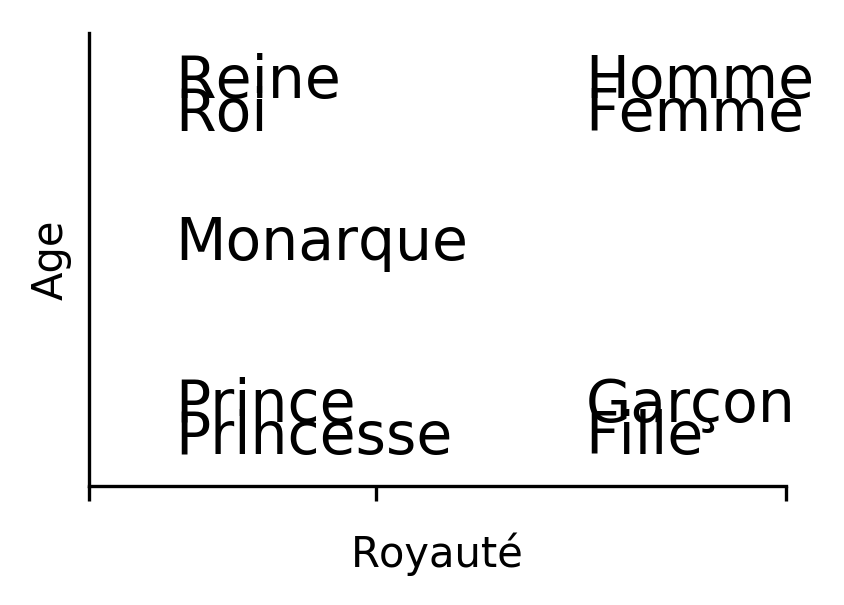
\includegraphics[width=\linewidth]{results/deep-learning/explanations/visualisation_embedding.png}
    \end{minipage}%
    \caption{Remplacement de l'encodage one-hot par une couche  embedding: cette couche permet de faire des rapprochements, que l'on peut représenter ensuite comme en troisième partie par une projection en deux dimensions (PCA). On se rend alors compte que la proximité de fortissimi et timendi a été apprise par la machine.}
\end{figure}